The \verb?Snd_Driver? module is a audio signal coder/decoder. It translates the signal between a parallel format and a bit serial format. The parallel format is sent to the \verb?Vol_Bal? module which processes the sound and sends it back. The bit serial format is used by the WM8731 chip. \verb?Snd_Driver? consists of two submodules: the \verb?Ctrl_Block? and two instances of the submodule \verb?Channel_Mod?. Depicted below (Figure \ref{fig:snddriver}), is a graphical representation of \verb?Snd_Driver?. 

\begin{figure}[H]
  \centering
  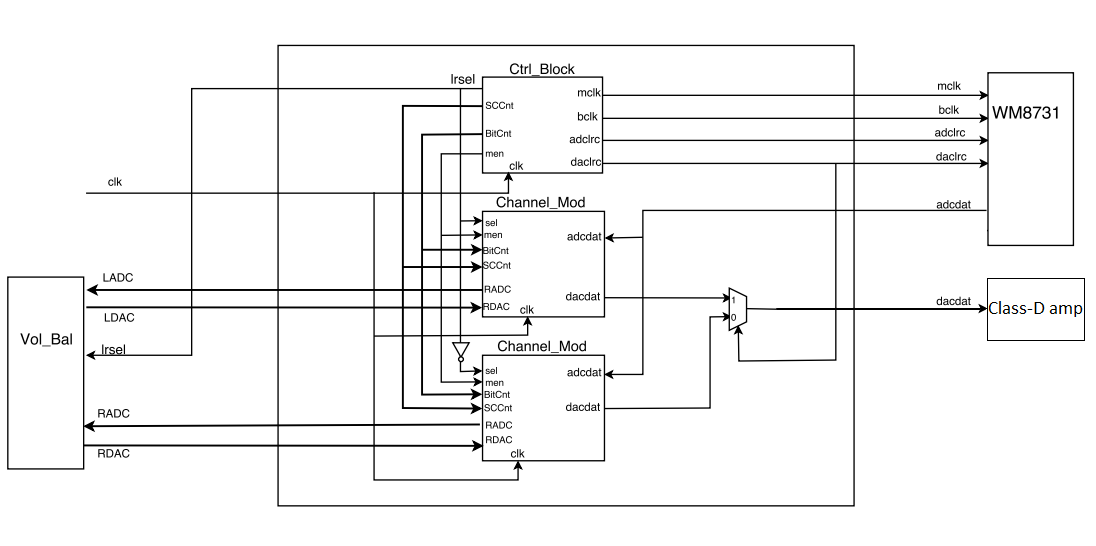
\includegraphics[scale=.40]{snddriver}
  \caption{Graphical representation of Snd\_Driver.}
  \label{fig:snddriver}
\end{figure}

\begin{figure}[H]
  \centering
  \caption{List of output signals}
  \label{tab:outputs}
    \begin{tabular}{|l|l|}     
      \hline
      \multicolumn{1}{|c|}{Name} & \multicolumn{1}{c|}{Description} \\
      \hline
      \verb=LADC/RADC= & Left/right outgoing samples for the \verb?Vol_Bal? module to process. 16-bits size.\\
      \hline
      \verb=lrsel= & Select signal for usage of left/right sample.\\
      \hline
      \verb=mclk/bclk= & \verb=mclk= is WM8731's internal operation clock, bclk is a bit clock\\
      \hline
      \verb=adclrc= & Left/right selector for \verb=adcdat=. \verb=adclrc==’1’ for left.\\
      \hline
      \verb=daclrc= & Left/right selector for \verb=dacdat=. \verb=daclrc==’1’ for left.\\
      \hline
      \verb=dacdat= & Serial bits to the DAC, one bit per \verb=bclk= pulse.\\
      \hline
    \end{tabular}
\end{figure}

\begin{figure}[H]
  \centering
  \label{tab:inputs}
  \caption{List of input signals}
    \begin{tabular}{|l|l|}     
        \hline
        \multicolumn{1}{|c|}{Name} & \multicolumn{1}{c|}{Description} \\
        \hline
        \verb=LDAC/RDAC= & Left/right incoming samples which shall be shifted out to the WM8731. 16-bits size.\\
        \hline
        \verb=adcdat= & Serial bits from the ADC, one bit per \verb=bclk= pulse.\\
        \hline
        \verb=clk= & The system clock. (50 MHz)\\
        \hline
    \end{tabular}
\end{figure}

\subsection{Snd\_Driver:Channel\_Mod}\label{sec:channelmod}

\verb?Channel_Mod? is a submodule instantiated twice, once for each bidirectional channel. One for the left and one for the right channel. The difference between the two is the \verb?sel?, or select, signal. One instance receives the \verb?sel? signal inverted. \verb?Channel_Mod? gets the \verb?sel? signal, which if active, indicates that the sound has been processed by \verb?Vol_Bal? for the selected channel and is ready to be sent back to WM8731. Depending on \verb?Sel?, \verb?Channel_Mod? shifts in/out the bits from/to \verb?adcdat?/\verb?dacdat?.

\subsection{Snd\_Driver:Ctrl\_Block}\label{sec:ctrlblock}

\verb?Ctrl_Block? acts as the control block of the module. It is responsible for generating several control signals. The module is built upon a 10-bit counter, \verb?cntr?. The control signals for the rest of the module is generated from different bits of \verb?cntr? in the \verb?Ctrl_Block?, essentially keeping track of what shall be done at which time.

